%!TEX program = xelatex
%# -*- coding: utf-8 -*-
%!TEX encoding = UTF-8 Unicode

\documentclass[12pt,oneside,a4paper]{article}\usepackage[]{graphicx}\usepackage[]{xcolor}
%% maxwidth is the original width if it is less than linewidth
%% otherwise use linewidth (to make sure the graphics do not exceed the margin)
\makeatletter
\def\maxwidth{ %
  \ifdim\Gin@nat@width>\linewidth
    \linewidth
  \else
    \Gin@nat@width
  \fi
}
\makeatother

\definecolor{fgcolor}{rgb}{0, 0, 0}
\newcommand{\hlnum}[1]{\textcolor[rgb]{0,0,0}{#1}}%
\newcommand{\hlstr}[1]{\textcolor[rgb]{0,0,1}{#1}}%
\newcommand{\hlcom}[1]{\textcolor[rgb]{0.443,0.478,0.702}{#1}}%
\newcommand{\hlopt}[1]{\textcolor[rgb]{0,0,0}{#1}}%
\newcommand{\hlstd}[1]{\textcolor[rgb]{0,0,0}{#1}}%
\newcommand{\hlkwa}[1]{\textcolor[rgb]{0.498,0,0.333}{\textbf{#1}}}%
\newcommand{\hlkwb}[1]{\textcolor[rgb]{0.498,0,0.333}{\textbf{#1}}}%
\newcommand{\hlkwc}[1]{\textcolor[rgb]{0.498,0,0.333}{\textbf{#1}}}%
\newcommand{\hlkwd}[1]{\textcolor[rgb]{0,0,0}{#1}}%

\usepackage{framed}
\makeatletter
\newenvironment{kframe}{%
 \def\at@end@of@kframe{}%
 \ifinner\ifhmode%
  \def\at@end@of@kframe{\end{minipage}}%
  \begin{minipage}{\columnwidth}%
 \fi\fi%
 \def\FrameCommand##1{\hskip\@totalleftmargin \hskip-\fboxsep
 \colorbox{shadecolor}{##1}\hskip-\fboxsep
     % There is no \\@totalrightmargin, so:
     \hskip-\linewidth \hskip-\@totalleftmargin \hskip\columnwidth}%
 \MakeFramed {\advance\hsize-\width
   \@totalleftmargin\z@ \linewidth\hsize
   \@setminipage}}%
 {\par\unskip\endMakeFramed%
 \at@end@of@kframe}
\makeatother

\definecolor{shadecolor}{rgb}{.97, .97, .97}
\definecolor{messagecolor}{rgb}{0, 0, 0}
\definecolor{warningcolor}{rgb}{1, 0, 1}
\definecolor{errorcolor}{rgb}{1, 0, 0}
\newenvironment{knitrout}{}{} % an empty environment to be redefined in TeX

\usepackage{alltt}
\usepackage{geometry}
\geometry{verbose,tmargin=2cm,bmargin=2cm,lmargin=2cm,rmargin=2cm}
\usepackage[pdfusetitle,
 bookmarks=true,bookmarksnumbered=true,bookmarksopen=true,bookmarksopenlevel=2,
 breaklinks=false,pdfborder={0 0 1},backref=false,colorlinks=false]
 {hyperref}
\hypersetup{pdfstartview={XYZ null null 1}}
\usepackage{url}
\setcounter{secnumdepth}{2}
\setcounter{tocdepth}{2}
\usepackage{microtype}

\usepackage{amsmath, amsthm, amssymb, amsfonts}
\usepackage[retainorgcmds]{IEEEtrantools}

\usepackage{algorithm}
\usepackage{algorithmic}
\renewcommand{\algorithmicrequire}{\textbf{Input:}} 
\renewcommand{\algorithmicensure}{\textbf{Output:}} 

\usepackage[sc]{mathpazo}
\linespread{1.1}
\usepackage[T1]{fontenc}


\usepackage{graphics}
\usepackage{graphicx}
\usepackage[figure]{hypcap}
\usepackage[hypcap]{caption}
\usepackage{tikz}
%\usepackage{grffile} 
%\usepackage{float} 
\usepackage{pdfpages}

\usepackage{multirow}
\usepackage{booktabs}
\usepackage{threeparttable}

%\usepackage[square,numbers,super,comma,sort]{natbib}
%\usepackage[backend=biber, style=nature, sorting=none, isbn=false, url=false, doi=false]{biblatex}
%\addbibresource{ref.bib}
%\usepackage[]{authblk}

\usepackage{verbatim}

\newcommand{\problem}[1]
{
    \clearpage
    \section*{Problem {#1}}
}

\newcommand{\subproblem}[1]
{
    \subsection*{Problem {#1}}
}


\newcommand{\solution}
{
    \vspace{15pt}
    \noindent\ignorespaces\textbf{\large Solution}
}

\usepackage{fancyhdr}
\usepackage{extramarks}
\lhead{\hmwkAuthorName}
\chead{\hmwkTitle}
\rhead{\firstxmark}
\cfoot{\thepage}

\newcommand{\hmwkTitle}{STAT 8051 HW 3}
\newcommand{\hmwkAuthorName}{Jingxiang Li}

\setlength\headheight{15pt}
\setlength\parindent{0pt}
\setlength{\parskip}{0.5em}

\newcommand{\m}[1]{\texttt{{#1}}}


\pagestyle{fancy}

\title{\hmwkTitle}
\author{\hmwkAuthorName}
\date{\today}
\IfFileExists{upquote.sty}{\usepackage{upquote}}{}
\begin{document}


\maketitle



\problem{6.7}
(Data file: \m{fuel2001}) With the fuel consumption data, consider the following two models in Wilkinson–Rogers notation:\\

\m{fuel $\sim$ Tax + Dlic + Income + log(Miles)} \hspace{50pt}     (6.22)\\
\m{fuel $\sim$ log(Miles) + Income + Dlic + Tax} \hspace{50pt}     (6.23)\\

These models are of course the same, as they only differ by the order in which the regressors are written.

\subproblem{6.7.1}
Show that the Type I anova for (6.22) and (6.23) are different. Provide an interpretation of each of the tests.

\solution
\begin{knitrout}
\definecolor{shadecolor}{rgb}{1, 1, 1}\color{fgcolor}\begin{kframe}
\begin{alltt}
\hlkwd{require}\hlstd{(alr4)}

\hlstd{data} \hlkwb{<-} \hlstd{fuel2001}
\hlstd{data}\hlopt{$}\hlstd{Dlic} \hlkwb{<-} \hlstd{data}\hlopt{$}\hlstd{Drivers} \hlopt{/} \hlstd{data}\hlopt{$}\hlstd{Pop}
\hlstd{data}\hlopt{$}\hlstd{Fuel} \hlkwb{<-} \hlnum{1000} \hlopt{*} \hlstd{data}\hlopt{$}\hlstd{FuelC} \hlopt{/} \hlstd{data}\hlopt{$}\hlstd{Pop}

\hlstd{m1} \hlkwb{<-} \hlkwd{lm}\hlstd{(Fuel} \hlopt{~} \hlstd{Tax} \hlopt{+} \hlstd{Dlic} \hlopt{+} \hlstd{Income} \hlopt{+} \hlkwd{log}\hlstd{(Miles),} \hlkwc{data} \hlstd{= data)}
\hlstd{m2} \hlkwb{<-} \hlkwd{lm}\hlstd{(Fuel} \hlopt{~} \hlkwd{log}\hlstd{(Miles)} \hlopt{+} \hlstd{Income} \hlopt{+} \hlstd{Dlic} \hlopt{+} \hlstd{Tax,} \hlkwc{data} \hlstd{= data)}
\hlkwd{anova}\hlstd{(m1)}
\end{alltt}
\begin{verbatim}
## Analysis of Variance Table
## 
## Response: Fuel
##            Df Sum Sq Mean Sq F value  Pr(>F)    
## Tax         1  26635   26635    6.33  0.0155 *  
## Dlic        1  79378   79378   18.85 7.7e-05 ***
## Income      1  61408   61408   14.58  0.0004 ***
## log(Miles)  1  34573   34573    8.21  0.0063 ** 
## Residuals  46 193700    4211                    
## ---
## Signif. codes:  0 '***' 0.001 '**' 0.01 '*' 0.05 '.' 0.1 ' ' 1
\end{verbatim}
\begin{alltt}
\hlkwd{anova}\hlstd{(m2)}
\end{alltt}
\begin{verbatim}
## Analysis of Variance Table
## 
## Response: Fuel
##            Df Sum Sq Mean Sq F value  Pr(>F)    
## log(Miles)  1  70478   70478   16.74 0.00017 ***
## Income      1  49996   49996   11.87 0.00123 ** 
## Dlic        1  63256   63256   15.02 0.00034 ***
## Tax         1  18264   18264    4.34 0.04287 *  
## Residuals  46 193700    4211                    
## ---
## Signif. codes:  0 '***' 0.001 '**' 0.01 '*' 0.05 '.' 0.1 ' ' 1
\end{verbatim}
\end{kframe}
\end{knitrout}

The above anova results are based on Type I anova. Note that all the main effects of predictors are significant in two models, however, the levels of significance are different in two models. suggesting that the order of predictors influence the result of Type I anova.

\subproblem{6.7.2}
Show that the Type II anova is the same for the two models. Which of the Type II tests are equivalent to Type I tests?

\solution
\begin{knitrout}
\definecolor{shadecolor}{rgb}{1, 1, 1}\color{fgcolor}\begin{kframe}
\begin{alltt}
\hlkwd{Anova}\hlstd{(}\hlkwc{mod} \hlstd{= m1,} \hlkwc{type} \hlstd{=} \hlnum{2}\hlstd{)}
\end{alltt}
\begin{verbatim}
## Anova Table (Type II tests)
## 
## Response: Fuel
##            Sum Sq Df F value  Pr(>F)    
## Tax         18264  1    4.34 0.04287 *  
## Dlic        56770  1   13.48 0.00063 ***
## Income      32940  1    7.82 0.00751 ** 
## log(Miles)  34573  1    8.21 0.00626 ** 
## Residuals  193700 46                    
## ---
## Signif. codes:  0 '***' 0.001 '**' 0.01 '*' 0.05 '.' 0.1 ' ' 1
\end{verbatim}
\begin{alltt}
\hlkwd{Anova}\hlstd{(}\hlkwc{mod} \hlstd{= m2,} \hlkwc{type} \hlstd{=} \hlnum{2}\hlstd{)}
\end{alltt}
\begin{verbatim}
## Anova Table (Type II tests)
## 
## Response: Fuel
##            Sum Sq Df F value  Pr(>F)    
## log(Miles)  34573  1    8.21 0.00626 ** 
## Income      32940  1    7.82 0.00751 ** 
## Dlic        56770  1   13.48 0.00063 ***
## Tax         18264  1    4.34 0.04287 *  
## Residuals  193700 46                    
## ---
## Signif. codes:  0 '***' 0.001 '**' 0.01 '*' 0.05 '.' 0.1 ' ' 1
\end{verbatim}
\end{kframe}
\end{knitrout}

Notice that the Type II anova is the same for the two models.

In the first model, the Type II test of \m{log(Miles)} is equal to Type I; in the second model, the Type II test of \m{Tax} is equal to the Type I test.

\problem{6.8}
Show that the overall F-test for multiple regression with an intercept can be written as
$$F = (\frac{n - p'}{p})\frac{R^{2}}{1-R^{2}}$$
Where $R^{2}$ is the proportion of variability explained by the regression. Thus, the F-statistic is just a transformation of $R^{2}$.

\solution

Following the definition of $R^{2}$ and $F$ statistic, we have
$$R^{2} = 1 - \frac{RSS}{SYY}$$
$$F = \frac{(SYY-RSS)/p}{RSS/(n - p - 1)}$$
Then 
$$\begin{aligned}
F & =\frac{SYY - RSS}{RSS} \cdot \frac{n - p - 1}{p}\\
& = \frac{1 - \frac{RSS}{SYY}}{\frac{RSS}{SYY}} \cdot \frac{n - p - 1}{p}\\
& = \frac{R^{2}}{1 - R^{2}} \cdot \frac{n - p - 1}{p}
\end{aligned}$$
Q.E.D.

\problem{6.9}
(Data file: \m{Cakes}) For the cakes data in Section 5.3.1, we fit the full second-order model,
$$E(Y|X_{1} = x_{1},X_{2} = x_{2}) = \beta_{0} + \beta_{1}x_{1} + \beta_{2}x_{1}^2 + \beta_{3}x_{2} + \beta_{4}x_{2}^{2} + \beta_{5}x_{1}x_{2}$$
Compute and summarize the following three hypothesis tests.

\begin{center}
NH: $\beta_{5} = 0$ vs. AH: $\beta_{5} \neq 0$

NH: $\beta_{2} = 0$ vs. AH: $\beta_{2} \neq 0$

NH: $\beta_{1} = \beta_{2} = \beta_{5} = 0$ vs. AH: Not all 0
\end{center}

\solution

\begin{knitrout}
\definecolor{shadecolor}{rgb}{1, 1, 1}\color{fgcolor}\begin{kframe}
\begin{alltt}
\hlstd{data} \hlkwb{<-} \hlstd{cakes}
\hlstd{m_full} \hlkwb{<-} \hlkwd{lm}\hlstd{(Y} \hlopt{~} \hlstd{(X1} \hlopt{+} \hlstd{X2)} \hlopt{^} \hlnum{2} \hlopt{+} \hlkwd{I}\hlstd{(X1} \hlopt{^} \hlnum{2}\hlstd{)} \hlopt{+} \hlkwd{I}\hlstd{(X2} \hlopt{^} \hlnum{2}\hlstd{),} \hlkwc{data} \hlstd{= data)}
\hlkwd{summary}\hlstd{(m_full)}
\end{alltt}
\begin{verbatim}
## 
## Call:
## lm(formula = Y ~ (X1 + X2)^2 + I(X1^2) + I(X2^2), data = data)
## 
## Residuals:
##    Min     1Q Median     3Q    Max 
## -0.491 -0.308  0.020  0.266  0.545 
## 
## Coefficients:
##              Estimate Std. Error t value Pr(>|t|)    
## (Intercept) -2.20e+03   2.42e+02   -9.13  1.7e-05 ***
## X1           2.59e+01   4.66e+00    5.56  0.00053 ***
## X2           9.92e+00   1.17e+00    8.50  2.8e-05 ***
## I(X1^2)     -1.57e-01   3.94e-02   -3.98  0.00408 ** 
## I(X2^2)     -1.20e-02   1.58e-03   -7.57  6.5e-05 ***
## X1:X2       -4.16e-02   1.07e-02   -3.88  0.00465 ** 
## ---
## Signif. codes:  0 '***' 0.001 '**' 0.01 '*' 0.05 '.' 0.1 ' ' 1
## 
## Residual standard error: 0.429 on 8 degrees of freedom
## Multiple R-squared:  0.949,	Adjusted R-squared:  0.917 
## F-statistic: 29.6 on 5 and 8 DF,  p-value: 5.86e-05
\end{verbatim}
\end{kframe}
\end{knitrout}

First Let's deal with the first two tests. Note that both of them are one coefficient two-sided t-test. Using R, it's easy to see the t-test result in the summary of full regression model. 

As the result, for the first hypothesis test, we see a tiny p-value of 0.0047, suggesting that we should reject the null hypothesis, $\beta_{5}$ should be non-zero.

Similarly, for the second test, we see a p-value of 0.0041, suggesting that $\beta_{2}$ should be non-zero, the null hypothesis should be rejected.

\begin{knitrout}
\definecolor{shadecolor}{rgb}{1, 1, 1}\color{fgcolor}\begin{kframe}
\begin{alltt}
\hlstd{m_test} \hlkwb{<-} \hlkwd{lm}\hlstd{(Y} \hlopt{~} \hlstd{X2} \hlopt{+} \hlkwd{I}\hlstd{(X2} \hlopt{^} \hlnum{2}\hlstd{),} \hlkwc{data} \hlstd{= data)}
\hlkwd{anova}\hlstd{(m_test, m_full)}
\end{alltt}
\begin{verbatim}
## Analysis of Variance Table
## 
## Model 1: Y ~ X2 + I(X2^2)
## Model 2: Y ~ (X1 + X2)^2 + I(X1^2) + I(X2^2)
##   Res.Df   RSS Df Sum of Sq    F  Pr(>F)    
## 1     11 11.47                              
## 2      8  1.47  3        10 18.1 0.00063 ***
## ---
## Signif. codes:  0 '***' 0.001 '**' 0.01 '*' 0.05 '.' 0.1 ' ' 1
\end{verbatim}
\end{kframe}
\end{knitrout}

Then we use anova to solve the last hypothesis test. the result shows a very tiny p-value, suggesting that the null hypothesis should be rejected, $\beta_{1}$, $\beta_{2}$ and $\beta_{5}$ are not all zero. 

\problem{6.14}
\textbf{Testing for lack-of-fit} (Data file: \m{MinnLand}) Refer to the Minnesota farm sales data introduced in Problem 5.4.

\subproblem{6.14.1}
Fit the regression model \m{log(acrePrice) $\sim$ year} via ols, where \m{year} is not a factor, but treated as a continuous predictor. What does this model say about the change in price per acre over time? Call this model A.

\solution
\begin{knitrout}
\definecolor{shadecolor}{rgb}{1, 1, 1}\color{fgcolor}\begin{kframe}
\begin{alltt}
\hlstd{data} \hlkwb{<-} \hlstd{MinnLand}
\hlstd{m_A} \hlkwb{<-} \hlkwd{lm}\hlstd{(}\hlkwd{log}\hlstd{(acrePrice)} \hlopt{~} \hlstd{year,} \hlkwc{data} \hlstd{= data)}
\hlkwd{coef}\hlstd{(m_A)}
\end{alltt}
\begin{verbatim}
## (Intercept)        year 
##   -193.8760      0.1005
\end{verbatim}
\end{kframe}
\end{knitrout}

model A says the \m{log(acrePrice)} increase 0.1005 per year on average.

\subproblem{6.14.2}

Fit the regression model via \m{log(acrePrice) $\sim$ 1  + fyear} via ols, where \m{fyear} is a factor with as many levels are there are years in the data, including the intercept in the model. What does this model say about the change in price per acre over time? Call this model B. (Hint: \m{fyear} is not included in the data file. You need to create it from the variable \m{year}.)

\solution
\begin{knitrout}
\definecolor{shadecolor}{rgb}{1, 1, 1}\color{fgcolor}\begin{kframe}
\begin{alltt}
\hlstd{data}\hlopt{$}\hlstd{fyear} \hlkwb{<-} \hlkwd{factor}\hlstd{(data}\hlopt{$}\hlstd{year)}
\hlstd{m_B} \hlkwb{<-} \hlkwd{lm}\hlstd{(}\hlkwd{log}\hlstd{(acrePrice)} \hlopt{~} \hlstd{fyear,} \hlkwc{data} \hlstd{= data)}
\hlkwd{coef}\hlstd{(m_B)}
\end{alltt}
\begin{verbatim}
## (Intercept)   fyear2003   fyear2004   fyear2005   fyear2006   fyear2007   fyear2008 
##     7.27175    -0.00155     0.14794     0.36026     0.39392     0.47682     0.68364 
##   fyear2009   fyear2010   fyear2011 
##     0.71407     0.75733     0.72071
\end{verbatim}
\end{kframe}
\end{knitrout}

In this model the intercept is the mean value of \m{log(acrePrice)} in 2002, and each coefficient of any other years represents the change of \m{log(acrePrice)} compared with that of 2002.

\subproblem{6.14.3}
Show that model A is a special case of model B, and so a hypothesis test of NH : model A versus AH : model B is reasonable.

\solution
\begin{knitrout}
\definecolor{shadecolor}{rgb}{1, 1, 1}\color{fgcolor}\begin{kframe}
\begin{alltt}
\hlstd{mean_value} \hlkwb{<-} \hlkwd{tapply}\hlstd{(}\hlkwc{X} \hlstd{=} \hlkwd{log}\hlstd{(data}\hlopt{$}\hlstd{acrePrice),} \hlkwc{INDEX} \hlstd{= data}\hlopt{$}\hlstd{year,} \hlkwc{FUN} \hlstd{= mean)}
\hlkwd{plot}\hlstd{(}\hlkwc{x} \hlstd{= data}\hlopt{$}\hlstd{year,} \hlkwc{y} \hlstd{=} \hlkwd{log}\hlstd{(data}\hlopt{$}\hlstd{acrePrice),} \hlkwc{col} \hlstd{=} \hlstr{"#A4A4A4"}\hlstd{,}
     \hlkwc{xlab} \hlstd{=} \hlstr{"year"}\hlstd{,} \hlkwc{ylab} \hlstd{=} \hlstr{"log(acrePrice)"}\hlstd{,} \hlkwc{main} \hlstd{=} \hlstr{"Model A VS. Model B"}\hlstd{)}
\hlkwd{lines}\hlstd{(}\hlkwc{x} \hlstd{=} \hlnum{2002}\hlopt{:}\hlnum{2011}\hlstd{,} \hlkwc{y} \hlstd{= mean_value,} \hlkwc{type} \hlstd{=} \hlstr{'b'}\hlstd{,} \hlkwc{pch} \hlstd{=} \hlnum{18}\hlstd{,} \hlkwc{cex} \hlstd{=} \hlnum{2}\hlstd{,} \hlkwc{lwd} \hlstd{=} \hlnum{2}\hlstd{,} \hlkwc{lty} \hlstd{=} \hlnum{2}\hlstd{)}
\hlkwd{abline}\hlstd{(}\hlkwd{coef}\hlstd{(m_A),} \hlkwc{lwd} \hlstd{=} \hlnum{2}\hlstd{,} \hlkwc{lty} \hlstd{=} \hlnum{1}\hlstd{)}
\hlkwd{legend}\hlstd{(}\hlstr{"topright"}\hlstd{,} \hlkwd{c}\hlstd{(}\hlstr{"Model A"}\hlstd{,} \hlstr{"Model B"}\hlstd{),} \hlkwc{lty} \hlstd{=} \hlkwd{c}\hlstd{(}\hlnum{1}\hlstd{,}\hlnum{2}\hlstd{),} \hlkwc{lwd} \hlstd{=} \hlkwd{c}\hlstd{(}\hlnum{2}\hlstd{,}\hlnum{2}\hlstd{),} \hlkwc{bg} \hlstd{=} \hlstr{"white"}\hlstd{)}
\end{alltt}
\end{kframe}

{\centering 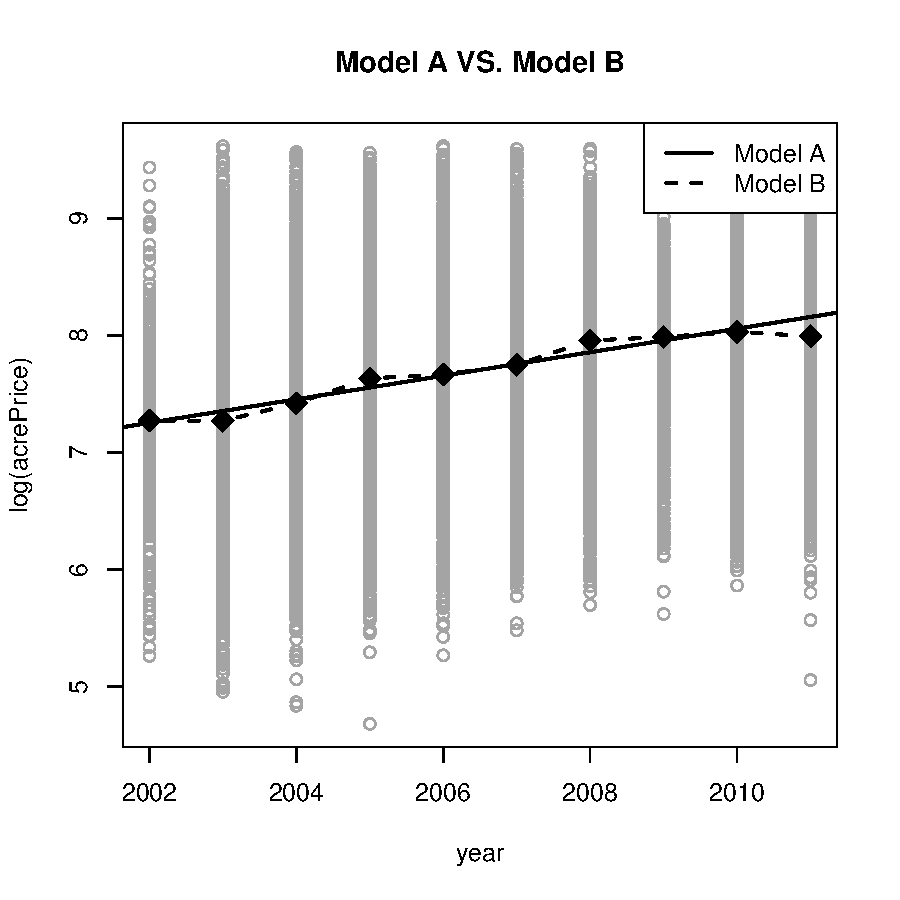
\includegraphics[width=.8\linewidth]{figure/p6143} 

}



\end{knitrout}

We show two fitted regression model in the graph above. Note that model B (dashed line in the graph above) can be viewed as a bunch of broken lines connected with each other on the mean value of response for each year; and model A (solid line in the graph above) can be viewed as a non-broken line go through all the points. Thus model A is just the special case of model B, if the mean values of response in each year are all on an unbroken line.

\subproblem{6.14.4}
A question of interest is whether or not model A provides an adequate description of the change in \m{log(acrePrice)} over time. The hypothesis test of NH : model A versus AH : model B addresses this question, and it can be called a \emph{lack-of-fit} test for model A. Perform the test and summarize results.

\solution

It's easy to find that $df_{A} = 18698$, $df_{B} = 18690$, $RSS_{A} = 8666.9333$, $RSS_{B} = 8579.2475$. Hence we can construct a F-statistic:
$$F = \frac{(RSS_{A} - RSS_{B}) / (df_{A} - df_{B})}{RSS_{B} / df_{B}} \sim~~F(df_{A} - df_{B}, df_{B})$$
So that we can use anova to do the \emph{lack-of-fit} test.
\begin{knitrout}
\definecolor{shadecolor}{rgb}{1, 1, 1}\color{fgcolor}\begin{kframe}
\begin{alltt}
\hlkwd{anova}\hlstd{(m_A, m_B)}
\end{alltt}
\begin{verbatim}
## Analysis of Variance Table
## 
## Model 1: log(acrePrice) ~ year
## Model 2: log(acrePrice) ~ fyear
##   Res.Df  RSS Df Sum of Sq    F Pr(>F)    
## 1  18698 8667                             
## 2  18690 8579  8      87.7 23.9 <2e-16 ***
## ---
## Signif. codes:  0 '***' 0.001 '**' 0.01 '*' 0.05 '.' 0.1 ' ' 1
\end{verbatim}
\end{kframe}
\end{knitrout}
Note that the p-value is very small, seems suggesting that we should reject NH, which means model A is lack of fit. However, the small p-value may result not from the model, but the huge sample size. Note that the sample size in this problem is 18700, and hence the power of this F-test is so big that even small differences in $RSS$ will result in large significance. In addition, from the graph we can see that, this two models are very close to each other. Therefore in this problem, though the F-test suggests very tiny p-value, it's very risky to reject the NH.

\problem{8.2}
(Data file: \m{stopping}) We reconsider the stopping distance data used in Problem 7.6.

\subproblem{8.2.1}
Using \m{Speed} as the only regressor, find an appropriate transformation for \m{Distance} that can linearize this regression.

\solution
\begin{knitrout}
\definecolor{shadecolor}{rgb}{1, 1, 1}\color{fgcolor}\begin{kframe}
\begin{alltt}
\hlkwd{require}\hlstd{(}\hlkwc{package} \hlstd{=} \hlstr{"gridExtra"}\hlstd{)}
\hlkwd{require}\hlstd{(}\hlkwc{package} \hlstd{=} \hlstr{"ggplot2"}\hlstd{)}
\hlstd{data} \hlkwb{<-} \hlstd{stopping}

\hlstd{p1} \hlkwb{<-} \hlkwd{ggplot}\hlstd{(data,} \hlkwd{aes}\hlstd{(}\hlkwc{x} \hlstd{= Speed,} \hlkwc{y} \hlstd{= Distance))}
\hlstd{p1} \hlkwb{<-} \hlstd{p1} \hlopt{+} \hlkwd{geom_point}\hlstd{()}
\hlstd{p1} \hlkwb{<-} \hlstd{p1} \hlopt{+} \hlkwd{geom_smooth}\hlstd{(}\hlkwc{formula} \hlstd{= y} \hlopt{~} \hlstd{x,} \hlkwc{method} \hlstd{=} \hlstr{"lm"}\hlstd{,} \hlkwc{se} \hlstd{=} \hlnum{FALSE}\hlstd{)}
\hlstd{p1} \hlkwb{<-} \hlstd{p1} \hlopt{+} \hlkwd{theme_bw}\hlstd{()} \hlopt{+} \hlkwd{theme}\hlstd{(}\hlkwc{text} \hlstd{=} \hlkwd{element_text}\hlstd{(}\hlkwc{size} \hlstd{=} \hlnum{14}\hlstd{))}
\hlstd{p1} \hlkwb{<-} \hlstd{p1} \hlopt{+} \hlkwd{ggtitle}\hlstd{(}\hlstr{"(a) Before Transformation"}\hlstd{)}

\hlstd{p2} \hlkwb{<-} \hlkwd{ggplot}\hlstd{(data,} \hlkwd{aes}\hlstd{(}\hlkwc{x} \hlstd{= Speed,} \hlkwc{y} \hlstd{=} \hlkwd{sqrt}\hlstd{(Distance)))}
\hlstd{p2} \hlkwb{<-} \hlstd{p2} \hlopt{+} \hlkwd{geom_point}\hlstd{()}
\hlstd{p2} \hlkwb{<-} \hlstd{p2} \hlopt{+} \hlkwd{geom_smooth}\hlstd{(}\hlkwc{formula} \hlstd{= y} \hlopt{~} \hlstd{x,} \hlkwc{method} \hlstd{=} \hlstr{"lm"}\hlstd{,} \hlkwc{se} \hlstd{=} \hlnum{FALSE}\hlstd{)}
\hlstd{p2} \hlkwb{<-} \hlstd{p2} \hlopt{+} \hlkwd{theme_bw}\hlstd{()} \hlopt{+} \hlkwd{theme}\hlstd{(}\hlkwc{text} \hlstd{=} \hlkwd{element_text}\hlstd{(}\hlkwc{size} \hlstd{=} \hlnum{14}\hlstd{))}
\hlstd{p2} \hlkwb{<-} \hlstd{p2} \hlopt{+} \hlkwd{ggtitle}\hlstd{(}\hlstr{"(b) After Transformation"}\hlstd{)}

\hlkwd{grid.arrange}\hlstd{(p1, p2,} \hlkwc{ncol}\hlstd{=}\hlnum{2}\hlstd{)}
\end{alltt}
\end{kframe}

{\centering 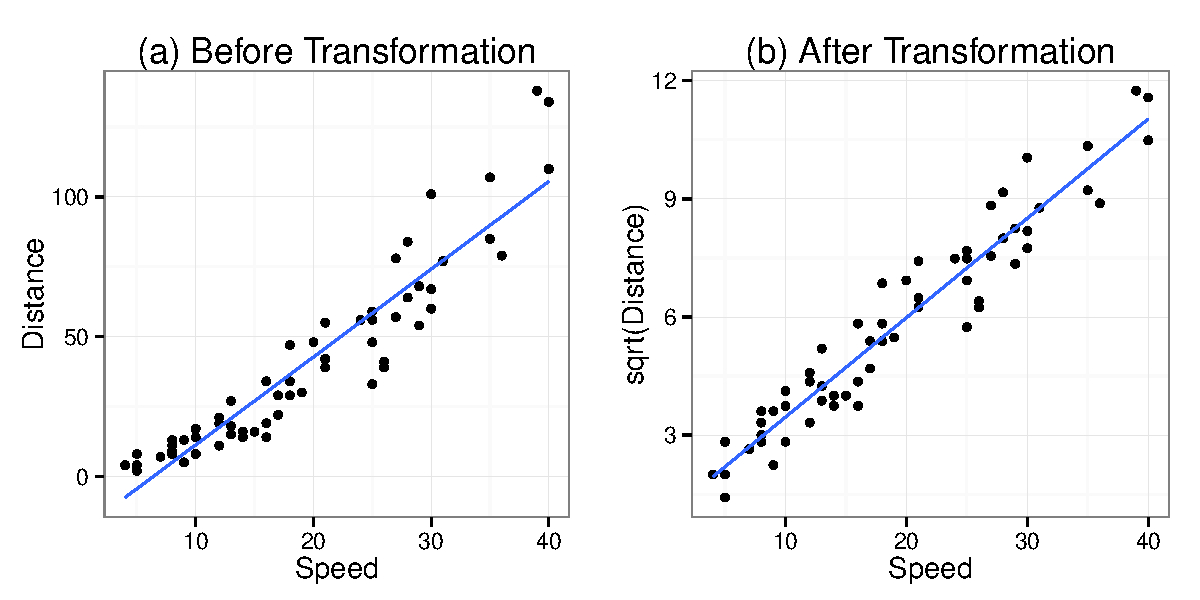
\includegraphics[width=.9\linewidth]{figure/p821} 

}



\end{knitrout}

We first draw the Scatterplot of \m{Distance} against \m{Speed}, as graph (a) above, and see that the relationship between response and predictor is approximately quadratic. Then let $\sqrt{\m{Speed}}$ as the new response and draw a new scatterplot (b), we see that the relationship between new response and predictor is almost linear. Thus the transformation we need should be square root.

\subproblem{8.2.2}
Using \m{Distance} as the response, transform the predictor \m{Speed} using a power transformation with each $\lambda \in \{-1,0,1\}$ and show that none of these transformations is adequate.

\solution
\begin{knitrout}
\definecolor{shadecolor}{rgb}{1, 1, 1}\color{fgcolor}\begin{kframe}
\begin{alltt}
\hlstd{p1} \hlkwb{<-} \hlkwd{ggplot}\hlstd{(data,} \hlkwd{aes}\hlstd{(}\hlkwc{x} \hlstd{= Speed,} \hlkwc{y} \hlstd{= Distance))}
\hlstd{p1} \hlkwb{<-} \hlstd{p1} \hlopt{+} \hlkwd{geom_point}\hlstd{()}
\hlstd{p1} \hlkwb{<-} \hlstd{p1} \hlopt{+} \hlkwd{geom_smooth}\hlstd{(}\hlkwc{formula} \hlstd{= y} \hlopt{~} \hlstd{x,} \hlkwc{method} \hlstd{=} \hlstr{"lm"}\hlstd{,} \hlkwc{se} \hlstd{=} \hlnum{FALSE}\hlstd{)}
\hlstd{p1} \hlkwb{<-} \hlstd{p1} \hlopt{+} \hlkwd{theme_bw}\hlstd{()} \hlopt{+} \hlkwd{theme}\hlstd{(}\hlkwc{text} \hlstd{=} \hlkwd{element_text}\hlstd{(}\hlkwc{size} \hlstd{=} \hlnum{14}\hlstd{))}
\hlstd{p1} \hlkwb{<-} \hlstd{p1} \hlopt{+} \hlkwd{ggtitle}\hlstd{(}\hlstr{"(a) Before Transformation"}\hlstd{)}

\hlstd{p2} \hlkwb{<-} \hlkwd{ggplot}\hlstd{(data,} \hlkwd{aes}\hlstd{(}\hlkwc{x} \hlstd{= Speed} \hlopt{-} \hlnum{1}\hlstd{,} \hlkwc{y} \hlstd{= Distance))}
\hlstd{p2} \hlkwb{<-} \hlstd{p2} \hlopt{+} \hlkwd{geom_point}\hlstd{()}
\hlstd{p2} \hlkwb{<-} \hlstd{p2} \hlopt{+} \hlkwd{geom_smooth}\hlstd{(}\hlkwc{formula} \hlstd{= y} \hlopt{~} \hlstd{x,} \hlkwc{method} \hlstd{=} \hlstr{"lm"}\hlstd{,} \hlkwc{se} \hlstd{=} \hlnum{FALSE}\hlstd{)}
\hlstd{p2} \hlkwb{<-} \hlstd{p2} \hlopt{+} \hlkwd{theme_bw}\hlstd{()} \hlopt{+} \hlkwd{theme}\hlstd{(}\hlkwc{text} \hlstd{=} \hlkwd{element_text}\hlstd{(}\hlkwc{size} \hlstd{=} \hlnum{14}\hlstd{))}
\hlstd{p2} \hlkwb{<-} \hlstd{p2} \hlopt{+} \hlkwd{ggtitle}\hlstd{(}\hlstr{"(b) lambda = 1"}\hlstd{)}

\hlstd{p3} \hlkwb{<-} \hlkwd{ggplot}\hlstd{(data,} \hlkwd{aes}\hlstd{(}\hlkwc{x} \hlstd{=} \hlkwd{log}\hlstd{(Speed),} \hlkwc{y} \hlstd{= Distance))}
\hlstd{p3} \hlkwb{<-} \hlstd{p3} \hlopt{+} \hlkwd{geom_point}\hlstd{()}
\hlstd{p3} \hlkwb{<-} \hlstd{p3} \hlopt{+} \hlkwd{geom_smooth}\hlstd{(}\hlkwc{formula} \hlstd{= y} \hlopt{~} \hlstd{x,} \hlkwc{method} \hlstd{=} \hlstr{"lm"}\hlstd{,} \hlkwc{se} \hlstd{=} \hlnum{FALSE}\hlstd{)}
\hlstd{p3} \hlkwb{<-} \hlstd{p3} \hlopt{+} \hlkwd{theme_bw}\hlstd{()} \hlopt{+} \hlkwd{theme}\hlstd{(}\hlkwc{text} \hlstd{=} \hlkwd{element_text}\hlstd{(}\hlkwc{size} \hlstd{=} \hlnum{14}\hlstd{))}
\hlstd{p3} \hlkwb{<-} \hlstd{p3} \hlopt{+} \hlkwd{ggtitle}\hlstd{(}\hlstr{"(c) lambda = 0"}\hlstd{)}

\hlstd{p4} \hlkwb{<-} \hlkwd{ggplot}\hlstd{(data,} \hlkwd{aes}\hlstd{(}\hlkwc{x} \hlstd{=} \hlopt{-}\hlstd{(Speed} \hlopt{^} \hlstd{(}\hlopt{-}\hlnum{1}\hlstd{)} \hlopt{-} \hlnum{1}\hlstd{),} \hlkwc{y} \hlstd{= Distance))}
\hlstd{p4} \hlkwb{<-} \hlstd{p4} \hlopt{+} \hlkwd{geom_point}\hlstd{()}
\hlstd{p4} \hlkwb{<-} \hlstd{p4} \hlopt{+} \hlkwd{geom_smooth}\hlstd{(}\hlkwc{formula} \hlstd{= y} \hlopt{~} \hlstd{x,} \hlkwc{method} \hlstd{=} \hlstr{"lm"}\hlstd{,} \hlkwc{se} \hlstd{=} \hlnum{FALSE}\hlstd{)}
\hlstd{p4} \hlkwb{<-} \hlstd{p4} \hlopt{+} \hlkwd{theme_bw}\hlstd{()} \hlopt{+} \hlkwd{theme}\hlstd{(}\hlkwc{text} \hlstd{=} \hlkwd{element_text}\hlstd{(}\hlkwc{size} \hlstd{=} \hlnum{14}\hlstd{))}
\hlstd{p4} \hlkwb{<-} \hlstd{p4} \hlopt{+} \hlkwd{ggtitle}\hlstd{(}\hlstr{"(d) lambda = -1"}\hlstd{)}

\hlkwd{grid.arrange}\hlstd{(p1, p2, p3, p4,} \hlkwc{ncol} \hlstd{=} \hlnum{2}\hlstd{,} \hlkwc{nrow} \hlstd{=} \hlnum{2}\hlstd{)}
\end{alltt}
\end{kframe}

{\centering 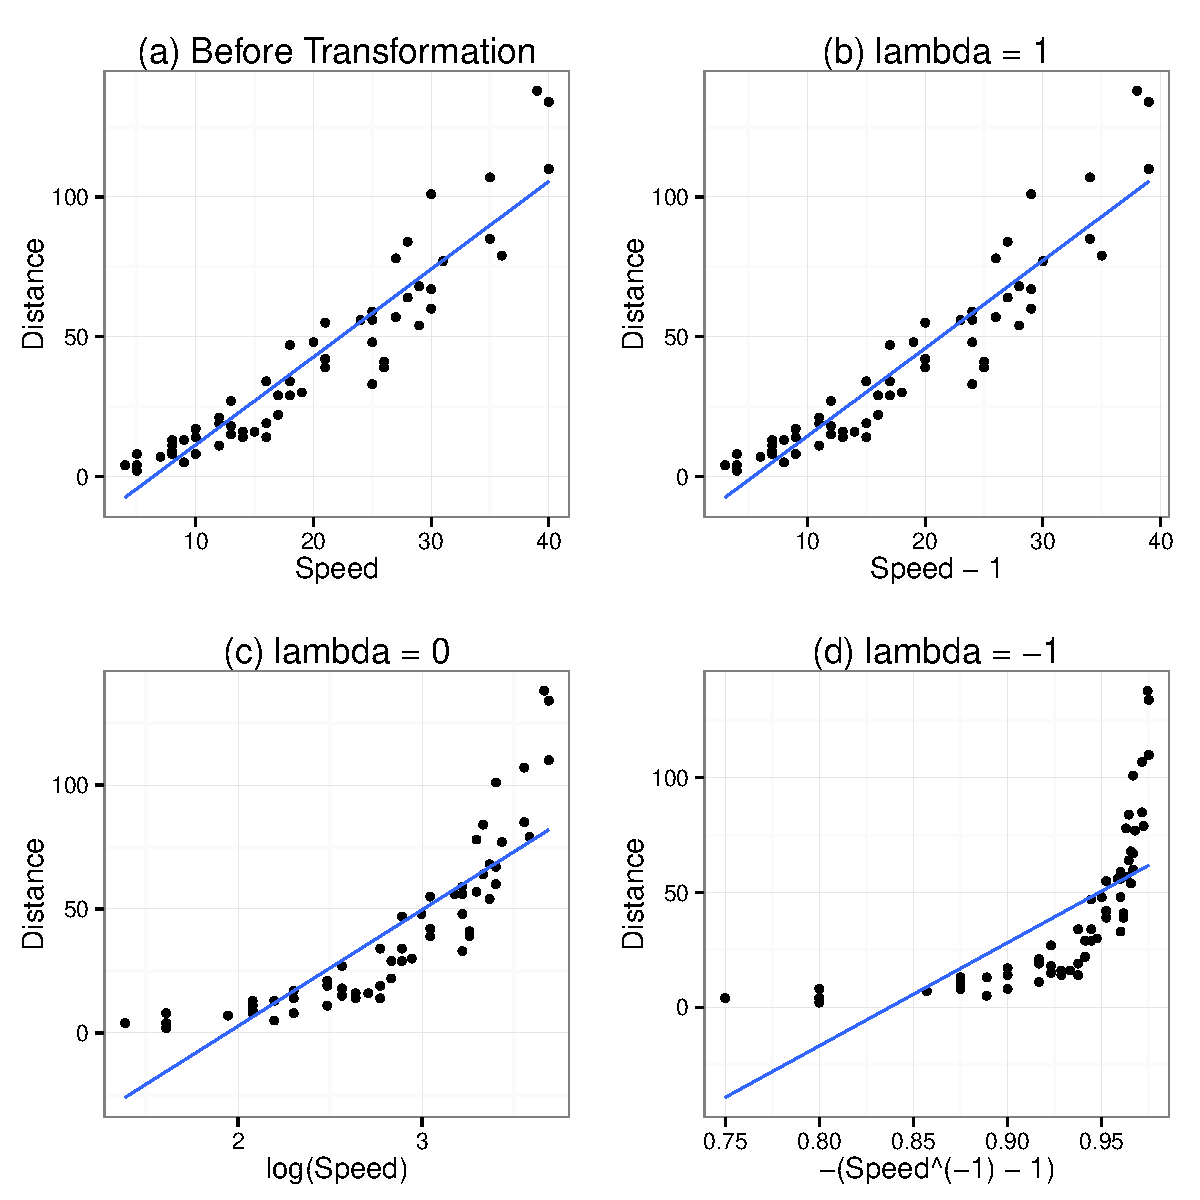
\includegraphics[width=.9\linewidth]{figure/p822} 

}



\end{knitrout}

graph (b), (c), (d) above are scatterplots where the predictor for each graph is respectively transformed with power $\lambda \in \{-1,0,1\}$. We can see that none of the above scatterplots can be well fitted by a linear model, suggesting that none of these transformations is adequate.

\subproblem{8.2.3}
Show that using $\lambda = 2$ does match the data well. This suggests using a quadratic polynomial for regressors, including both \m{Speed} and $\m{Speed}^2$.

\solution
\begin{knitrout}
\definecolor{shadecolor}{rgb}{1, 1, 1}\color{fgcolor}\begin{kframe}
\begin{alltt}
\hlstd{p1} \hlkwb{<-} \hlkwd{ggplot}\hlstd{(data,} \hlkwd{aes}\hlstd{(}\hlkwc{x} \hlstd{= (Speed} \hlopt{^} \hlnum{2} \hlopt{-} \hlnum{1}\hlstd{)}\hlopt{/}\hlnum{2}\hlstd{,} \hlkwc{y} \hlstd{= Distance))}
\hlstd{p1} \hlkwb{<-} \hlstd{p1} \hlopt{+} \hlkwd{geom_point}\hlstd{()}
\hlstd{p1} \hlkwb{<-} \hlstd{p1} \hlopt{+} \hlkwd{geom_smooth}\hlstd{(}\hlkwc{formula} \hlstd{= y} \hlopt{~} \hlstd{x,} \hlkwc{method} \hlstd{=} \hlstr{"lm"}\hlstd{,} \hlkwc{se} \hlstd{=} \hlnum{FALSE}\hlstd{)}
\hlstd{p1} \hlkwb{<-} \hlstd{p1} \hlopt{+} \hlkwd{theme_bw}\hlstd{()} \hlopt{+} \hlkwd{theme}\hlstd{(}\hlkwc{text} \hlstd{=} \hlkwd{element_text}\hlstd{(}\hlkwc{size} \hlstd{=} \hlnum{12}\hlstd{))}
\hlstd{p1} \hlkwb{<-} \hlstd{p1} \hlopt{+} \hlkwd{ggtitle}\hlstd{(}\hlstr{"lambda = 2"}\hlstd{)}
\hlstd{p1}
\end{alltt}
\end{kframe}

{\centering 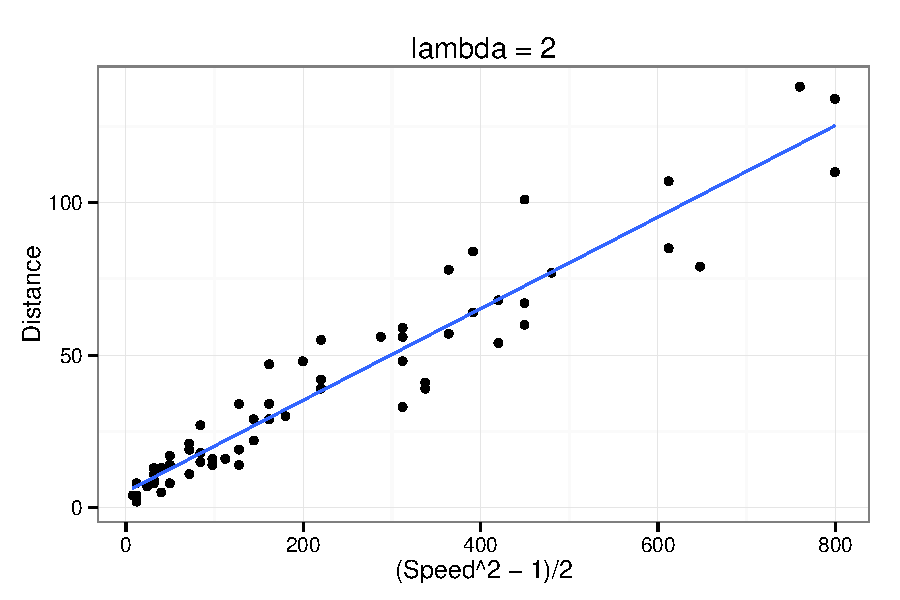
\includegraphics[width=.8\linewidth]{figure/p823} 

}



\end{knitrout}

The graph above is the scatterplot of \m{Distance} against \m{Speed}, where \m{Speed} is transformed with $\lambda = 2$. It shows that under such transformation, the points can be fitted well by a linear model.

\subproblem{8.2.4}
Hald (1960) suggested on the basis of a theoretical argument using a quadratic mean function for \m{Distance} given \m{Speed}, with $\mathrm{Var}(\m{Distance}|\m{Speed})=\sigma^{2}\m{Speed}^2$. Draw the plot of \m{Distance} versus \m{Speed}, and add a line on the plot of the fitted curve from Hald’s model. Then obtain the fitted values from the fit of the transformed \m{Distance} on \m{Speed}, using the transformation you found in Problem 8.2.1. Transform these fitted values to the \m{Distance} scale (for example, if you fit the regression \m{sqrt(Distance)} $\sim$ \m{Speed}, then the fitted values would be in square-root scale and
you would square them to get the original \m{Distance} scale). Add to your plot the line corresponding to these transformed fitted values. Compare the fit of the two models.

\solution
\begin{knitrout}
\definecolor{shadecolor}{rgb}{1, 1, 1}\color{fgcolor}\begin{kframe}
\begin{alltt}
\hlkwd{require}\hlstd{(reshape2)}
\hlstd{data} \hlkwb{<-} \hlstd{stopping}
\hlstd{m_h} \hlkwb{<-} \hlkwd{lm}\hlstd{(Distance} \hlopt{~} \hlkwd{I}\hlstd{(Speed}\hlopt{^}\hlnum{2}\hlstd{),} \hlkwc{data} \hlstd{= data,} \hlkwc{weights} \hlstd{= Speed}\hlopt{^}\hlnum{2}\hlstd{)}
\hlstd{m_1} \hlkwb{<-} \hlkwd{lm}\hlstd{(}\hlkwd{sqrt}\hlstd{(Distance)} \hlopt{~} \hlstd{Speed,} \hlkwc{data} \hlstd{= data)}

\hlstd{x} \hlkwb{=} \hlnum{0}\hlopt{:}\hlnum{45}
\hlstd{y_h} \hlkwb{=} \hlstd{x}\hlopt{^}\hlnum{2} \hlopt{*} \hlkwd{coef}\hlstd{(m_h)[}\hlnum{2}\hlstd{]} \hlopt{+} \hlkwd{coef}\hlstd{(m_h)[}\hlnum{1}\hlstd{]}
\hlstd{y_1} \hlkwb{=} \hlstd{(x} \hlopt{*} \hlkwd{coef}\hlstd{(m_1)[}\hlnum{2}\hlstd{]} \hlopt{+} \hlkwd{coef}\hlstd{(m_1)[}\hlnum{1}\hlstd{])}\hlopt{^}\hlnum{2}

\hlstd{data_plot} \hlkwb{<-} \hlkwd{data.frame}\hlstd{(x,} \hlkwc{y_Hald} \hlstd{= y_h,} \hlkwc{y_P1} \hlstd{= y_1)}
\hlstd{data_plot} \hlkwb{<-} \hlkwd{melt}\hlstd{(data_plot,} \hlkwc{id.vars} \hlstd{=} \hlnum{1}\hlstd{)}
\hlkwd{colnames}\hlstd{(data_plot)[}\hlnum{2}\hlstd{]} \hlkwb{<-} \hlstr{"group"}

\hlstd{p} \hlkwb{<-} \hlkwd{ggplot}\hlstd{()}
\hlstd{p} \hlkwb{<-} \hlstd{p} \hlopt{+} \hlkwd{geom_point}\hlstd{(}\hlkwd{aes}\hlstd{(}\hlkwc{x} \hlstd{= data}\hlopt{$}\hlstd{Speed,} \hlkwc{y} \hlstd{= data}\hlopt{$}\hlstd{Distance))}
\hlstd{p} \hlkwb{<-} \hlstd{p} \hlopt{+} \hlkwd{geom_line}\hlstd{(}\hlkwd{aes}\hlstd{(}\hlkwc{x} \hlstd{= data_plot}\hlopt{$}\hlstd{x,} \hlkwc{y} \hlstd{= data_plot}\hlopt{$}\hlstd{value,}
                       \hlkwc{linetype} \hlstd{= data_plot}\hlopt{$}\hlstd{group))}
\hlstd{p} \hlkwb{<-} \hlstd{p} \hlopt{+} \hlkwd{theme_bw}\hlstd{()} \hlopt{+} \hlkwd{theme}\hlstd{(}\hlkwc{text} \hlstd{=} \hlkwd{element_text}\hlstd{(}\hlkwc{size} \hlstd{=} \hlnum{16}\hlstd{))}
\hlstd{p} \hlkwb{<-} \hlstd{p} \hlopt{+} \hlkwd{ggtitle}\hlstd{(}\hlstr{"Distance VS. Speed"}\hlstd{)} \hlopt{+} \hlkwd{xlab}\hlstd{(}\hlstr{"Speed"}\hlstd{)} \hlopt{+} \hlkwd{ylab}\hlstd{(}\hlstr{"Distance"}\hlstd{)}
\hlstd{p} \hlkwb{<-} \hlstd{p} \hlopt{+} \hlkwd{scale_linetype_discrete}\hlstd{(}\hlkwc{name}  \hlstd{=}\hlstr{"Model"}\hlstd{,}
                              \hlkwc{breaks}\hlstd{=}\hlkwd{c}\hlstd{(}\hlstr{"y_Hald"}\hlstd{,} \hlstr{"y_P1"}\hlstd{),}
                              \hlkwc{labels}\hlstd{=}\hlkwd{c}\hlstd{(}\hlstr{"Hald Model"}\hlstd{,} \hlstr{"Problem 8.2.1"}\hlstd{))}
\hlstd{p}
\end{alltt}
\end{kframe}

{\centering 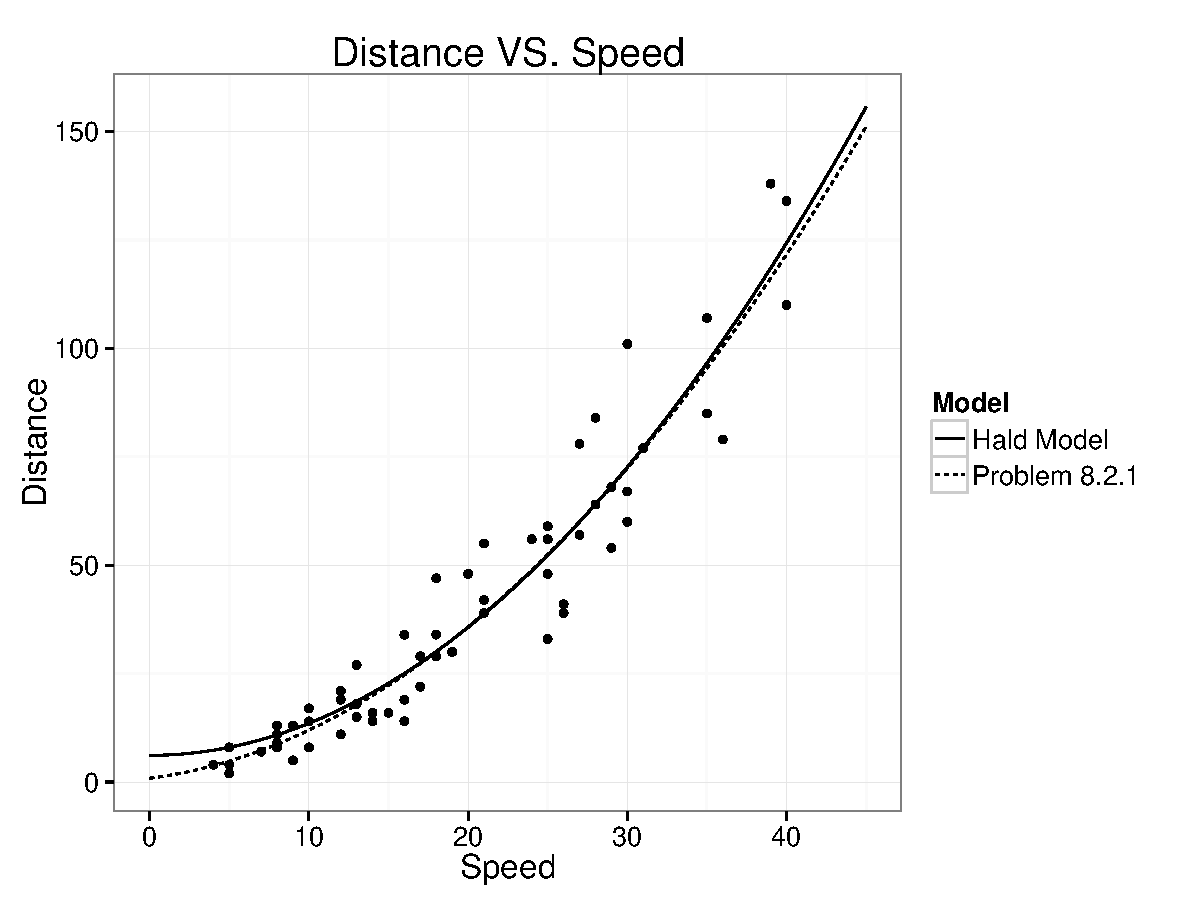
\includegraphics[width=.8\linewidth]{figure/p824} 

}



\end{knitrout}

In this problem we fit Hold's model with weighted parameter $\m{Speed}^2$, and then draw the Hold's model and model fitted in problem 8.2.1 in the same graph above. We see that, according to the graph above, these two models are almost the same. The only difference is that Hold's model is better in fitting points where predictor value is high, and model in problem 8.2.1 is better in fitting points where predictor value is low.

\problem{9.11}
(Data file: \m{fuel2001}) In the fuel consumption data, consider fitting the mean function
$$E(\m{Fuel}|X) = \beta_{0} + \beta_{1}\m{Tax} + \beta_{2}\m{Dlic} + \beta_{3}\m{Income} + \beta_{4}\m{log(Miles)}$$
For this regression, we find $\hat{\sigma} = 64.891$ with 46 $df$, and the diagnostic statistics for four states and the District of Columbia were the following:

\begin{table}[ht!]
\centering
%\caption*{Problem 9.11}
\begin{tabular}{lrrr}
\toprule
 \multicolumn{1}{c}{  } & \multicolumn{1}{c}{ \m{Fuel} } & \multicolumn{1}{c}{ $\hat{e}_{i}$ } & \multicolumn{1}{c}{ $h_{ii}$ } \\
\midrule
 Alaska & $514.279$ & $-163.145$ & $0.256$ \\
 New York & $374.164$ & $-137.599$ & $0.162$ \\
 Hawaii & $426.349$ & $-102.409$ & $0.206$ \\
 Wyoming & $842.792$ & $183.499$ & $0.084$ \\
 District of Columbia & $317.492$ & $-49.452$ & $0.415$ \\
\bottomrule
\end{tabular}
\end{table}

Compute $D_{i}$ and $t_{i}$ for each of these cases, and test for one outlier. Which is most influential?

\solution
\begin{knitrout}
\definecolor{shadecolor}{rgb}{1, 1, 1}\color{fgcolor}\begin{kframe}
\begin{alltt}
\hlstd{data} \hlkwb{<-} \hlstd{fuel2001}
\hlstd{data}\hlopt{$}\hlstd{Dlic} \hlkwb{<-} \hlstd{data}\hlopt{$}\hlstd{Drivers} \hlopt{/} \hlstd{data}\hlopt{$}\hlstd{Pop}
\hlstd{data}\hlopt{$}\hlstd{Fuel} \hlkwb{<-} \hlnum{1000} \hlopt{*} \hlstd{data}\hlopt{$}\hlstd{FuelC} \hlopt{/} \hlstd{data}\hlopt{$}\hlstd{Pop}

\hlstd{test_outlier} \hlkwb{<-} \hlkwa{function}\hlstd{(}\hlkwc{data}\hlstd{,} \hlkwc{index}\hlstd{)}
\hlstd{\{}
    \hlstd{m_tmp} \hlkwb{<-} \hlkwd{lm}\hlstd{(Fuel} \hlopt{~} \hlstd{Tax} \hlopt{+} \hlstd{Dlic} \hlopt{+} \hlstd{Income} \hlopt{+} \hlkwd{log}\hlstd{(Miles),} \hlkwc{data} \hlstd{= data,}
                \hlkwc{x} \hlstd{=} \hlnum{TRUE}\hlstd{,} \hlkwc{y} \hlstd{=} \hlnum{TRUE}\hlstd{)}
    \hlstd{X} \hlkwb{=} \hlstd{m_tmp}\hlopt{$}\hlstd{x}
    \hlstd{y} \hlkwb{=} \hlstd{m_tmp}\hlopt{$}\hlstd{y}

    \hlstd{m} \hlkwb{<-} \hlkwd{lm}\hlstd{(Fuel} \hlopt{~} \hlstd{Tax} \hlopt{+} \hlstd{Dlic} \hlopt{+} \hlstd{Income} \hlopt{+} \hlkwd{log}\hlstd{(Miles),} \hlkwc{data} \hlstd{= data,} \hlkwc{subset} \hlstd{=} \hlopt{-}\hlstd{index)}
    \hlstd{y_predict} \hlkwb{<-} \hlkwd{predict}\hlstd{(}\hlkwc{object} \hlstd{= m,} \hlkwc{newdata} \hlstd{= data[index, ])}

    \hlstd{sigma} \hlkwb{<-} \hlkwd{sqrt}\hlstd{(}\hlkwd{sum}\hlstd{(m}\hlopt{$}\hlstd{residuals}\hlopt{^}\hlnum{2}\hlstd{)} \hlopt{/} \hlstd{m}\hlopt{$}\hlstd{df.residual)}
    \hlstd{t} \hlkwb{=} \hlstd{(y[index]} \hlopt{-} \hlstd{y_predict)} \hlopt{/}
        \hlstd{(sigma} \hlopt{*} \hlkwd{sqrt}\hlstd{(}\hlnum{1} \hlopt{+} \hlkwd{t}\hlstd{(X[index, ])} \hlopt \hlkwd{solve}\hlstd{(}\hlkwd{t}\hlstd{(X[}\hlopt{-}\hlstd{index, ])}
                                \hlopt \hlstd{X[}\hlopt{-}\hlstd{index, ])} \hlopt \hlstd{X[index, ]))}
    \hlstd{p_value} \hlkwb{=} \hlstd{(}\hlnum{1} \hlopt{-} \hlkwd{pt}\hlstd{(}\hlkwd{abs}\hlstd{(t),} \hlkwc{df} \hlstd{= m}\hlopt{$}\hlstd{df.residual))} \hlopt{*} \hlnum{2}
    \hlkwd{data.frame}\hlstd{(t, p_value)}
\hlstd{\}}

\hlstd{test_influence} \hlkwb{<-} \hlkwa{function}\hlstd{(}\hlkwc{data}\hlstd{,} \hlkwc{index}\hlstd{)}
\hlstd{\{}
    \hlstd{m_full} \hlkwb{<-} \hlkwd{lm}\hlstd{(Fuel} \hlopt{~} \hlstd{Tax} \hlopt{+} \hlstd{Dlic} \hlopt{+} \hlstd{Income} \hlopt{+} \hlkwd{log}\hlstd{(Miles),} \hlkwc{data} \hlstd{= data)}
    \hlstd{m_noindex} \hlkwb{<-} \hlkwd{lm}\hlstd{(Fuel} \hlopt{~} \hlstd{Tax} \hlopt{+} \hlstd{Dlic} \hlopt{+} \hlstd{Income} \hlopt{+} \hlkwd{log}\hlstd{(Miles),}
                    \hlkwc{data} \hlstd{= data,} \hlkwc{subset} \hlstd{=} \hlopt{-}\hlstd{index)}

    \hlstd{y_predict_full} \hlkwb{<-} \hlkwd{predict}\hlstd{(}\hlkwc{object} \hlstd{= m_full,} \hlkwc{newdata} \hlstd{= data)}
    \hlstd{y_predict_noindex} \hlkwb{<-} \hlkwd{predict}\hlstd{(}\hlkwc{object} \hlstd{= m_noindex,} \hlkwc{newdata} \hlstd{= data)}

    \hlstd{sigma_2} \hlkwb{<-} \hlkwd{sum}\hlstd{(m_full}\hlopt{$}\hlstd{residuals}\hlopt{^}\hlnum{2}\hlstd{)} \hlopt{/} \hlstd{m_full}\hlopt{$}\hlstd{df.residual}

    \hlstd{D} \hlkwb{<-} \hlkwd{t}\hlstd{(y_predict_full} \hlopt{-} \hlstd{y_predict_noindex)} \hlopt
        \hlstd{(y_predict_full} \hlopt{-} \hlstd{y_predict_noindex)} \hlopt{/}
        \hlstd{(}\hlkwd{length}\hlstd{(}\hlkwd{coef}\hlstd{(m_full))} \hlopt{*} \hlstd{sigma_2)}

    \hlkwd{data.frame}\hlstd{(D)}
\hlstd{\}}

\hlstd{result} \hlkwb{<-} \hlkwd{rbind}\hlstd{(}\hlkwd{test_outlier}\hlstd{(data,} \hlkwd{match}\hlstd{(}\hlstr{"AK"}\hlstd{,} \hlkwd{rownames}\hlstd{(data))),}
\hlkwd{test_outlier}\hlstd{(data,} \hlkwd{match}\hlstd{(}\hlstr{"NY"}\hlstd{,} \hlkwd{rownames}\hlstd{(data))),}
\hlkwd{test_outlier}\hlstd{(data,} \hlkwd{match}\hlstd{(}\hlstr{"HI"}\hlstd{,} \hlkwd{rownames}\hlstd{(data))),}
\hlkwd{test_outlier}\hlstd{(data,} \hlkwd{match}\hlstd{(}\hlstr{"WY"}\hlstd{,} \hlkwd{rownames}\hlstd{(data))),}
\hlkwd{test_outlier}\hlstd{(data,} \hlkwd{match}\hlstd{(}\hlstr{"DC"}\hlstd{,} \hlkwd{rownames}\hlstd{(data))))}

\hlstd{result} \hlkwb{<-} \hlkwd{cbind}\hlstd{(result,} \hlkwd{rbind}\hlstd{(}\hlkwd{test_influence}\hlstd{(data,} \hlkwd{match}\hlstd{(}\hlstr{"AK"}\hlstd{,} \hlkwd{rownames}\hlstd{(data))),}
\hlkwd{test_influence}\hlstd{(data,} \hlkwd{match}\hlstd{(}\hlstr{"NY"}\hlstd{,} \hlkwd{rownames}\hlstd{(data))),}
\hlkwd{test_influence}\hlstd{(data,} \hlkwd{match}\hlstd{(}\hlstr{"HI"}\hlstd{,} \hlkwd{rownames}\hlstd{(data))),}
\hlkwd{test_influence}\hlstd{(data,} \hlkwd{match}\hlstd{(}\hlstr{"WY"}\hlstd{,} \hlkwd{rownames}\hlstd{(data))),}
\hlkwd{test_influence}\hlstd{(data,} \hlkwd{match}\hlstd{(}\hlstr{"DC"}\hlstd{,} \hlkwd{rownames}\hlstd{(data)))))}

\hlkwd{rownames}\hlstd{(result)} \hlkwb{<-} \hlkwd{c}\hlstd{(}\hlstr{"AK"}\hlstd{,} \hlstr{"NY"}\hlstd{,} \hlstr{"HI"}\hlstd{,} \hlstr{"WY"}\hlstd{,} \hlstr{"DC"}\hlstd{)}
\hlstd{result}
\end{alltt}
\begin{verbatim}
##          t  p_value      D
## AK -3.1930 0.002570 0.5850
## NY -2.4382 0.018771 0.2081
## HI -1.8144 0.076291 0.1624
## WY  3.2461 0.002212 0.1596
## DC -0.9962 0.324475 0.1408
\end{verbatim}
\end{kframe}
\end{knitrout}

Here we define two functions \m{test\_outlier} and \m{test\_influence} to get the $D_{i}$, $t_{i}$ and the p-value derived from $t_{i}$. The p-values derived from the outlier test suggest that points representing Alaska, New York and Wyoming are outliers. The most influential point is Alaska.













\end{document}
